\chapter{Theoretische Grundlagen}
In diesem Kapitel werden die für die Realisierung benötigten Technologien und
Methoden beschrieben.

Dazu wird zuerst erklärt, was man unter NoSql versteht und eine kurze Zeitlinie
der Entwicklung. Anschließend werden die verschiedenen Arten von NoSql und
speziell von Schlüssel-Wert-Systemen beschrieben.

Danach folgt der Vergleich von Redis, Memcached und Voldemort. Dazu werden
zuerst die jeweiligen Systeme erläutert. Anschließend folgt der eigentliche
Vergleich, dazu werden die jeweiligen Eigenschaften kurz erläutert und danach
wie die jeweiligen Systeme dies umsetzen.

\section{NoSql}
NoSql-Systeme sind keine neue Erfindung, sondern entwickelten sich quasi
parallel mit den relationalen Systemen. Der Grund warum erst jetzt NoSql einen
so großen Durchbruch erfährt, hängt vor allem mit dem BigData-Gedanken zusammen.
Vor BigData war es üblich die Geschäftsdaten auf wenigen Datenbank-Server zu
speichern. Mit der Entwicklung der Sozialen-Netzwerke und der zunehmenden
Vernetzung von Alltagsgegenständen stieg die erzeugte Datenmenge rapide auf
Peta-, Exa-Byte Bereich an. Dies hatte zur Folge, dass sich die Geschäftsdaten
mit herkömmlichen Mitteln nicht mehr effektiv Speichern und verarbeiten ließen
und man nach Alternativen gesucht hat, den NoSql-Systemen.
Obwohl der NoSql Begriff heute so eine Aktualität besitzt, gibt es keine
einheitliche Begriffsdefinition. Vielmehr ist NoSql ähnlich wie \gls{AJAX} ein
Sammelbegriff für verschiedene Technologien und Ideen. Während früher NoSql
wörtlich für „no Sql“ also "kein Sql" stand steht es heute eher
für „not only Sql“ also "nicht nur Sql". Auch ab wann man ein System als
NoSql-System zählt, ist nicht klar geregelt. Vielmehr gibt es eine Reihe von
Punkten, die ein System erfüllen kann wie: \cite{Edlich2011}

\begin{itemize}
    \item Das zugrundeliegende Datenmodell ist nicht relational.
    \item Die System sind von Anbeginn auf eine verteilelte und horizontale
        Skallierbarkeit ausgerichtet.
    \item Das NoSql-System ist Open-Source.
    \item Das System ist schemafrei oder hat nur schwache Schemarestriktionen.
    \item Aufgrund der verteielten Architektur unterstützt das System einfache
        Datenreplikation.
    \item Das System besitz eine einfache \gls{API}.
    \item Dem System liegt meist auch ein anderes Konsitenzmodell zugrunde:
        Eventuelly Consistenz und \gls{BASE} aber nicht \gls{ACID}.
\end{itemize}

. Daraus haben sich die unterschiedlichsten Systeme entwickelt.

\subsection{Entwicklungsmeilensteine}
Der Ursprung von NoSql ist die im Jahr 1979 von Ken Thompson entwickelte
Datenbank DBM\footnote{\url{http://www.gnu.org/software/gdbm/gdbm.html}}, die
bis heute noch von Linux verwendet wird. Die ersten NoSql Datenbanken, die
heute noch existieren entstanden in den 80er-Jahren, wie
Lotus Note\footnote{\url{http://www-03.ibm.com/software/products/de/ibmdomino}},
BerkleyDB\footnote{\url{http://www.oracle.com/us/products/database/berkeley-db/index.html}},
GT.M\footnote{\url{https://sourceforge.net/projects/fis-gtm/https://sourceforge.net/projects/fis-gtm/}},~\dots .
Der Begriff NoSql wurde das erste Mal 1998 von Carlo Strozzi benutzt, der eine
relationale Datenbank entwickelt hatte jedoch ohne Sql. Der richtige Durchbruch
kam allerdings erst im Jahr 2000 mit dem Web 2.0 und den daraus resultierenden
Anstieg des Datenvolumens. Dieser Datenanstieg erforderte neue Methoden zur
effizienteren Speicherung und Verarbeitung. Google war dabei der Vorreiter mit
seinem Map-/Reduce-Ansatz. Die Idee dabei ist es, eine große Datenmenge in
kleinere Pakete aufzuteilen und diese dann unabhängig voneinander zu verarbeiten.
Anschließend werden die einzelnen Zwischenergebnisse gesammelt und zu einem
Gesamtergebnis zusammengefasst. Diese Idee ließ sich sehr gut mit den Ideen
der funktionalen Programmiersprachen umsetzen, denn dort wird auf einer Kopie
der tatsächlichen Daten gearbeitet. Später zogen die anderen großen Firmen mit
eigenen Lösungen nach und heute kann man sagen, dass es den Map-/Reduce-Ansatz
nicht mehr gibt, sondern verschiedene Implementierungen, die für einen gewissen
Einsatzzweck entwickelt wurden. Die Entwicklung der modernen NoSql-Systemen
begann im Jahr 2005 mit Systemen wie Neo4j\footnote{\url{http://www.neo4j.com}},
Redis\footnote{\url{http://www.redis.io}},
Cassandra\footnote{\url{http://cassandra.apache.org}},~\dots{} und hält bis
heute noch an.

\subsection{Arten von NoSql-Systemen}
Wie oben schon beschrieben existieren eine Vielzahl an unterschiedlichsten
NoSql-Systemen. Dies hat zur Folge, dass es nicht leicht ist das für seinen
Anwendungsfall passende System zu finden. Deshalb kam der Gedanke NoSql-Systeme
nach bestimmten Kriterien zu sortieren um eine bessere Entscheidung treffen zu
können. Schnell entwickelten sich mehrere Kriterien. Die gröbste Einteilung,
die man vorgenommen hat, war die Einteilung in Kern-NoSql-Systeme und
Soft-NoSql-Systemen. Wobei die Grenze und der Unterschied zwischen den Gruppen
nicht klar geregelt ist. Danach werden NoSql-Systeme häufig nach ihrem
zugrundeliegenden Datenmodell eingeteilt. Nachfolgend eine Einteilung der
NoSql-Systeme nach dem Datenmodell mit einer Erklärung was man sich unter dem
jeweiligen Typ vorzustellen hat und einige Vertreter davon:

\begin{itemize}
    \item Kern-NoSql-Systeme
        \begin{description}
            \item[dokumentenbasierte Systeme] Dokumentenbasierte System
                speichern die Daten in Dateien, meist im \gls{JSON}-Format, ab.
                Zu dieser Gruppe gehören Systeme wie MongoDB oder CouchDB.
            \item[Schlüssel-Wert-Systeme] Schlüssel-Wert-Systeme speichern wie
                der Name schon sagt die Daten unter einem gewissen Schlüssel ab,
                über den dann später die Daten wieder gelesen werden. Zu dieser
                Gruppe gehören Systeme wie Redis, Voldemort, Memcached.
            \item[graphbasierte Systeme] Bei graphbasierten Systemen liegen die
                Daten als Graph vor. Solche Systeme ermöglichen es leicht
                herauszufinden, welcher Knoten mit einem anderen Knoten in
                Beziehung steht. Dies wird bei Sozialennetzwerken bezutzt um
                herauszufinden, wer "Freund" von jemanden ist. Zu dieser Gruppe
                gehören Systeme wie Neo4j.
            \item[spaltenorientierte Systeme] Spaltenorientiert System haben
                Ähnlichkeiten mit relationalen Systemen, die ja auch über
                Spalten verfügen. Allerdings kann man bei einem
                spaltenorientierten System eine Liste von Schlüssel-Wert-Paaren
                abspeichern und im Extremfall kann sogar die Spalte eine Liste
                von Schlüssel-Wert-Paaren sein. Zu dieser Gruppe gehören Systeme
                wie HBase, Cassandra.
        \end{description}
    \item Soft-NoSql-Systeme
        \begin{description}
            \item[XML-Datenbanken] XML-Datenbanken sind spezielle
                dokumentenbasierte Systeme bei denen statt \gls{JSON}-Dateien
                \gls{XML}-Dateien benutzt werden.
            \item[Objekt-Datenbanken] Objekt-Datenbanken speichern
                Objektstrukturen ab. Vorraussetzung ist allerdings, das die
                Objekte serialisierbar sind. Werden solche Objekt-Datenbanken
                anstelle von relationalen Datenbanken eingesetzt, dann kann man
                sich den Einsatz von \gls{ORM}-Frameworks wie
                Hibernate\footnote{\url{http://www.hibernate.org}}
                oder EclipseLink\footnote{\url{http://www.eclipse.org/eclipselink}}
                sparen.
        \end{description}
\end{itemize}

. Im weiteren Verlauf werden wir nur noch Schlüssel-Wert-Systeme betrachten.

\section{Schlüssel-Wert-Systeme}
Schlüssel-Wert-Systeme sind Systeme, die wie der Name schon sagt, einen Wert,
also die Daten unter einem bestimmten Schlüssel ablegen. Der Zugriff auf den
abgelegten Wert erfolgt anschließend ebenfalls über den Schlüssel. Die Schlüssel
und die Werte können dabei ganz verschiedene Formen aufweisen. Die Schlüssel
sind im einfachsten Fall einfache Zeichenketten mit einer spezifischen Länge.
Andere Systeme lassen erst einmal oder mehrmals einen Hash-Algorithmus über den
Daten laufen und nehmen die erzeugte Hash-Summe als Schlüssel. Auch die Werte
sind im einfachsten Fall einfache Zeichenketten, jedoch können manche Systeme
auch komplexere Datenstrukturen wie Listen, Mengen, Wörterbücher,~\dots{}
speichern. Wenn man die Geschwindigkeit der Operationen betrachtet, dann stellt
man fest, dass die Lese-Operation schnell ist, vorausgesetzt man kennt den
Schlüssel und die Schreib-Operation langsam. Die Schlüssel-Wert-Systeme lassen
sich nochmals in verschiedene Gruppen einteilen, wobei jede Gruppe eine
Eigenschaft fokussiert.

\subsubsection{Arten von Schlüssel-Wert-Systemen}
Schlüssel-Wert-Systeme lassen sich in Gruppen einteilen. Dabei hat jede Gruppen
eine spezifische Eigenschaft. Diese Einteilung ist aber keineswegs fest, sondern
ein System kann durchaus auch mehreren Gruppen angehören, je nachdem wie seine
aktuelle Konfiguration ist. Die folgende Liste spezifieziert die möglichen
Gruppen:

\begin{description}
    \item[Caches] \gls{RAM}-basierte Systeme oder Caches halten ihre gesamten
        Daten im \gls{RAM} vor. Deshalb werden sie oft als Zwischenspeicher
        benutzt. Dies hat zur Folge, falls ein Server ausfällt sind die Daten
        entgültig weg. Ein beliebter Anwendungsfall ist es solch ein System
        zwischen der Anwendung und dem Datenbankserver zu schalten und die
        Ergebnisse der Datenbankanfragen für spätere Zugriffe zwischen
        zuspeichern. Zu dieser Gruppe gehören Systeme wie Memcached.
    \item[Festplatten-Systeme] Festplatten-Systeme arbeiten im Prinzip wie Caches
        nur mit der Einschränkung, dass sie ihre Daten nicht im \gls{RAM} halten
        sondern auf der Festplatte. Außerdem legen solche Systeme oft
        Wiederherstellungsdateien an. Damit sind solche Systeme gut gegen
        Ausfälle geschützt. Zu dieser Gruppe gehören Systeme wie Redis.
    \item[Sortierte Schlüssel-Wert-Systeme] Sortierte Schlüssel-Wert-System
        verfügen über Ordnungs- und Sortierfunktionen auf den Schlüsseln.
        Außerdem gibt es System die die Schlüssel in einer Extra Index-Tabelle
        speichern. Zu dieser Gruppe gehören Systeme wie BerkleyDB.
    \item[Eventual Consistence-Systeme] Solche Systeme stellen sicher, dass das
        System nach einer gewissen Dauer wieder in einem konsistenten Zustand
        ist. Zu dieser Gruppe gehören Systeme wie Voldemort.
\end{description}

. Nachfolgend folgt der allgemeine Überblick über die drei ausgewählten Systeme
Memcached, Redis und Voldemort.

\subsection{Memcached}
Memcached ist ein NoSql-System und gehört in die Gruppe der
Schlüssel-Wert-Systeme und in die Untergruppe der Caches 
\begin{quote}
   „Free \& open source, high-performance, distributed memory object caching
    system [\dots]" \cite{Memcached2015}
\end{quote}
. Memcached wurde im Jahr 2003 von Brad Fitzpatrick bei der Firma Danga
Interactive heute Say Media für die Webseite LiveJournal entwickelt. Die
aktuelle Version ist die Version 1.5.0. Die ersten Versionen von Memcached
waren in Perl geschrieben. Später wurde der Memcached in C neugeschrieben. Der
Vorteil von Memcached liegt in der Beschleunigung von Webseiten in dem es
Datenbank-, Webservice- und Templateergenbisse zwischenspeichert 
\begin{quote}
    „[\dots{}] but intended for use in speeding up dynamic web
applications by alleviating database load. Memcached is an in-memory key-value
store for small chunks of arbitrary data (strings, objects) from results of
database calls, API calls, or page rendering." \cite{Memcached2015}
\end{quote}
.

Memcached arbeitet nach einem Client-Server-Modell siehe dazu auch die
Abbildung \ref{fig:memcached-architecture}. Zunächst läuft auf dem
Server bzw. den Servern ein Dienst oder mehrere. Der Zugriff erfolgt dann über
eine Bibliothek für die jeweilige Programmiersprache. Sobald Daten geschrieben
oder gelesen werden sollen, berechnet die Bibliothek aus der Anfrage eine
Hash-Summe, welche den Server identifieziert, welcher die Anfrage bekommen
soll. Dieser verarbeitet dann die Anfrage und gibt die Daten zurück oder
speichert die Daten unter einer neu berechneten Hash-Summe

\begin{quote}
    „Zunächst nimmt die Client-Bibliothek den Schlüssel und errechnet aus ihm
    mit einer ausgeklügelten, mathematischen Funktion eine Zahl, den so
    genannten Hashwert. Diese Nummer sagt der Bibliothek, an welchen
    Memcached-Daemon sie sich wenden muss. Nachdem dieser alle Daten erhalten
    hat, errechnet er mit einer eigenen Hashfunktion die Speicherstelle, unter
    der er die Daten schließlich einlagert." \cite{Schuermann2009}
\end{quote}
.

\begin{figure}
\centering
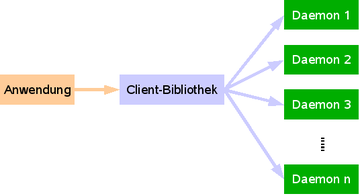
\includegraphics{images/memcached_illustration_large.png}
\caption{Architektur von Memcached \cite{Schuermann2009}}
\label{fig:memcached-architecture}
\end{figure}

Memcached hat zwei verschiedene Protokolle, welche zur Kommunikation benutzt
werden können Text-Protokoll und Binär-Protokoll. Diese Protokolle machen
spezielle Einschränkungen auf den Schlüssel. Die maximale Schlüssellänge ist
immer 250 Zeichen lang und die Protokolle definieren, welche Zeichen erlaubt
sind als Schlüssel. Als Werte lassen sich einfache Zeichenketten oder
Binärdaten ablegen. Dies hat zur Folge, dass Memcached nicht direkt ein
Datenbankergebnis speichern kann, sondern dies erst von der Anwendung in eine
serialisierbare Struktur gepackt werden muss. Außerdem muss die Anwendung
wissen, was sich für Datentypen hinter den einzelnen Schlüssel verbergen.
Die maximale Größe ist dabei standartmäßig 64 MB, dies lässt allerdings
konfigurieren. Jedoch sollte die Größe immer kleiner sein als
der \gls{RAM}-Speicher des Memcached-Dienstes mit dem kleinsten
zugewiesenen \gls{RAM}.

\subsection{Redis}
Redis ist ebenfalls ein Schlüssel-Wert-System, gehört aber normalerweise in die
Untergruppe der Festplatten-Systeme. Redis lässt sich jedoch auch in die Gruppe
der Cache-Systeme eintragen, wenn eine bestimmte Konfiguration benutzt wird.
Im Normalbetrieb hällt Redis seine Daten im \gls{RAM} und legt in bestimmten
Abständen einen Zwischenstand auf der Festplatte ab. Wenn man Redis in der
Konfiguration als reinen Cache laufen lässt, dann werden keine Zwischenstände
abgelegt und Redis würde sich dann so wie Memcached verhalten
\begin{quote}
    „In order to achieve its outstanding performance, Redis works with an
    in-memory dataset. Depending on your use case, you can persist it either by
    dumping the dataset to disk every once in a while, or by appending each
    command to a log. Persistence can be optionally disabled, if you just need
    a feature-rich, networked, in-memory cache.“ \cite{Redis2010}
\end{quote}
. Redis wurde im Jahr 2009 von Salvatore Sanfilippo bei Redis Labs entwickelt.
Die aktuelle Version ist 4.0.1. Redis ist komplett in C geschrieben.
Redis läuft ebenfalls nach einem Client-Server-Modell, jedoch mit dem
Unterschied, dass immer nur eine Redis-Dienst läuft. Der Zugriff auf den Server
erfolgt ebenfalls über die Client-Bibliothek. Der wichtigste Unterschied
zwischen Redis und Memcached sind die erlaubten Schlüssel und Werte. Wie schon
oben erwähnt sind Schlüssel in Memcached immer Zeichenketten mit einer
maximalen Länge von 250 Zeichen. Im Gegensatz dazu existiert diese Einschränkung
bei Redis nicht. Dort ist es ohne Probleme möglich auch ein Bild als Schlüssel
zu verwenden
\begin{quote}
    „Redis keys are binary safe, this means that you can use any binary sequence
    as a key, from a string like ‚foo‘ to the content of a JPEG file. The empty
    string is also a valid key. [\dots]“ \cite{Redis2010}
\end{quote}
. Der Schlüssel wie auch die Werte dürfen lediglich die 512 MB Grenze nicht
überschreiten. Bei den zulässigen Werten unterscheidet sich Redis stark von den
anderen Systemen. Während Memcached nur Zeichenketten oder serialisierte Objekte
speichern kann ist Redis in der Lage mit Listen, Mengen und Wörterbüchern direkt
umzugehen.
